\chapter{Experimentelle Untersuchungen}
\chaptermark{Experimentelle Untersuchungen}  % short form for headlines on pages
\label{ch:EntwickelteMethode}

\section{Angewendete Methodik}
\subsection{Testumgebung}
\subsection{Benchmark Script}

\section{Ergebnisse}

\subsection{Apple M1 Pro}

\begin{figure}[H]
\centering
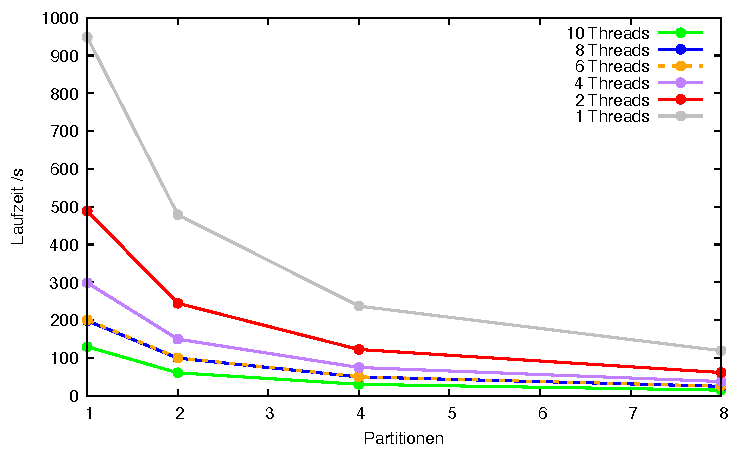
\includegraphics[width=0.8\textwidth]{../results/plots/m1pro/comp_all_threads.pdf}
\caption{Ergebnisse der Leistungstests verglichen nach Thread Anzahl}
\label{fig:m1pro_benchmark_threads}
\end{figure}

\begin{figure}[htbp!]
\centering
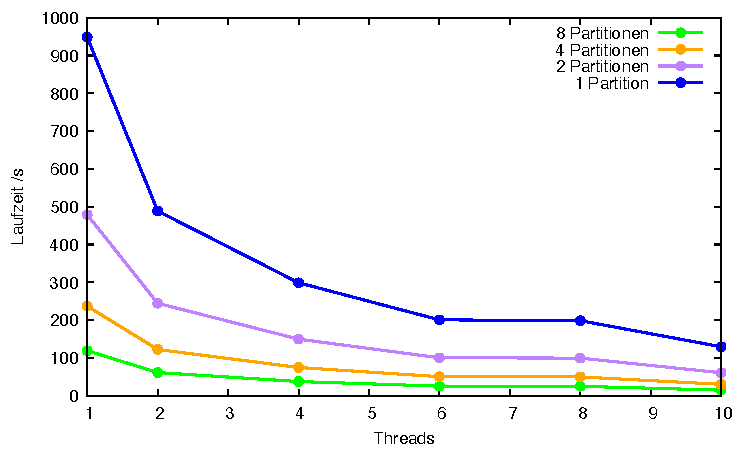
\includegraphics[width=0.8\textwidth]{../results/plots/m1pro/comp_all_partitions.pdf}
\caption{Ergebnisse der Leistungstests verglichen nach Datensatzgröße}
\label{fig:m1pro_benchmark_partitions}
\end{figure}

\subsection{AMD Ryzen 3600XT}

\begin{figure}[htbp!]
\centering
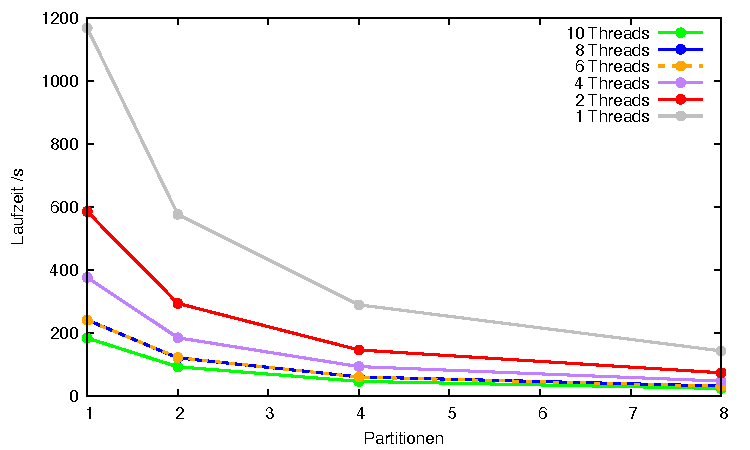
\includegraphics[width=0.8\textwidth]{../results/plots/3600xt/comp_all_threads.pdf}
\caption{Ergebnisse der Leistungstests verglichen nach Thread Anzahl}
\label{fig:ryzen_benchmark_threads}
\end{figure}

\begin{figure}[htbp!]
\centering
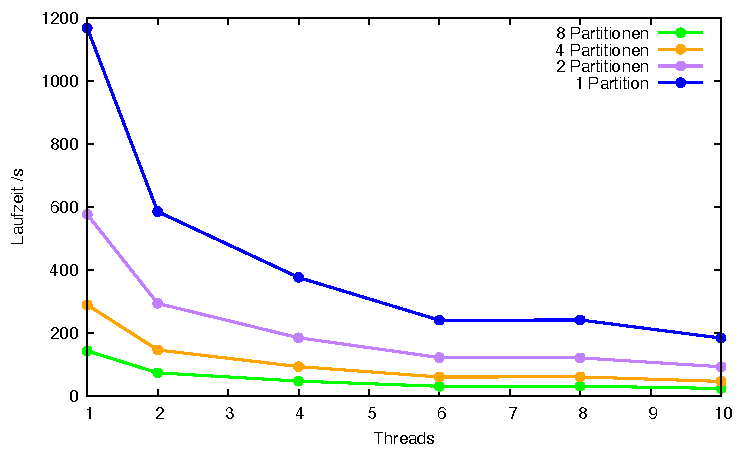
\includegraphics[width=0.8\textwidth]{../results/plots/3600xt/comp_all_partitions.pdf}
\caption{Ergebnisse der Leistungstests verglichen nach Datensatzgröße}
\label{fig:ryzen_benchmark_partitions}
\end{figure}

\subsection{Raspberry Pi 3}

\begin{figure}[htbp!]
\centering
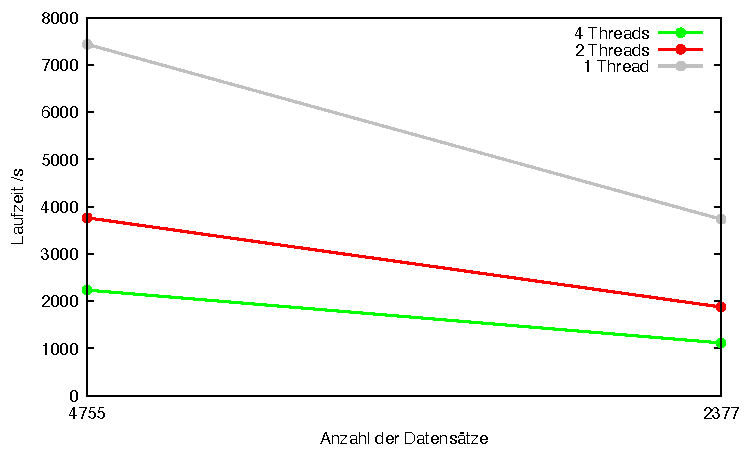
\includegraphics[width=0.8\textwidth]{../results/plots/raspberrypi3/comp_all_threads.pdf}
\caption{Ergebnisse der Leistungstests verglichen nach Thread Anzahl}
\label{fig:raspi_benchmark_threads}
\end{figure}

\begin{figure}[htbp!]
\centering
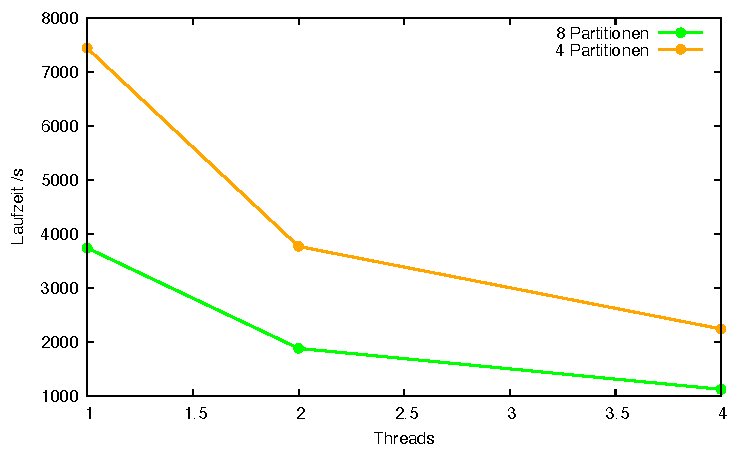
\includegraphics[width=0.8\textwidth]{../results/plots/raspberrypi3/comp_all_partitions.pdf}
\caption{Ergebnisse der Leistungstests verglichen nach Datensatzgröße}
\label{fig:raspi_benchmark_partitions}
\end{figure}

\subsection{Cloud Server}

\section{Auswertung}

\newpage
